\documentclass{standalone}
\usepackage{tikz}
\usetikzlibrary{patterns, positioning}


\begin{document}
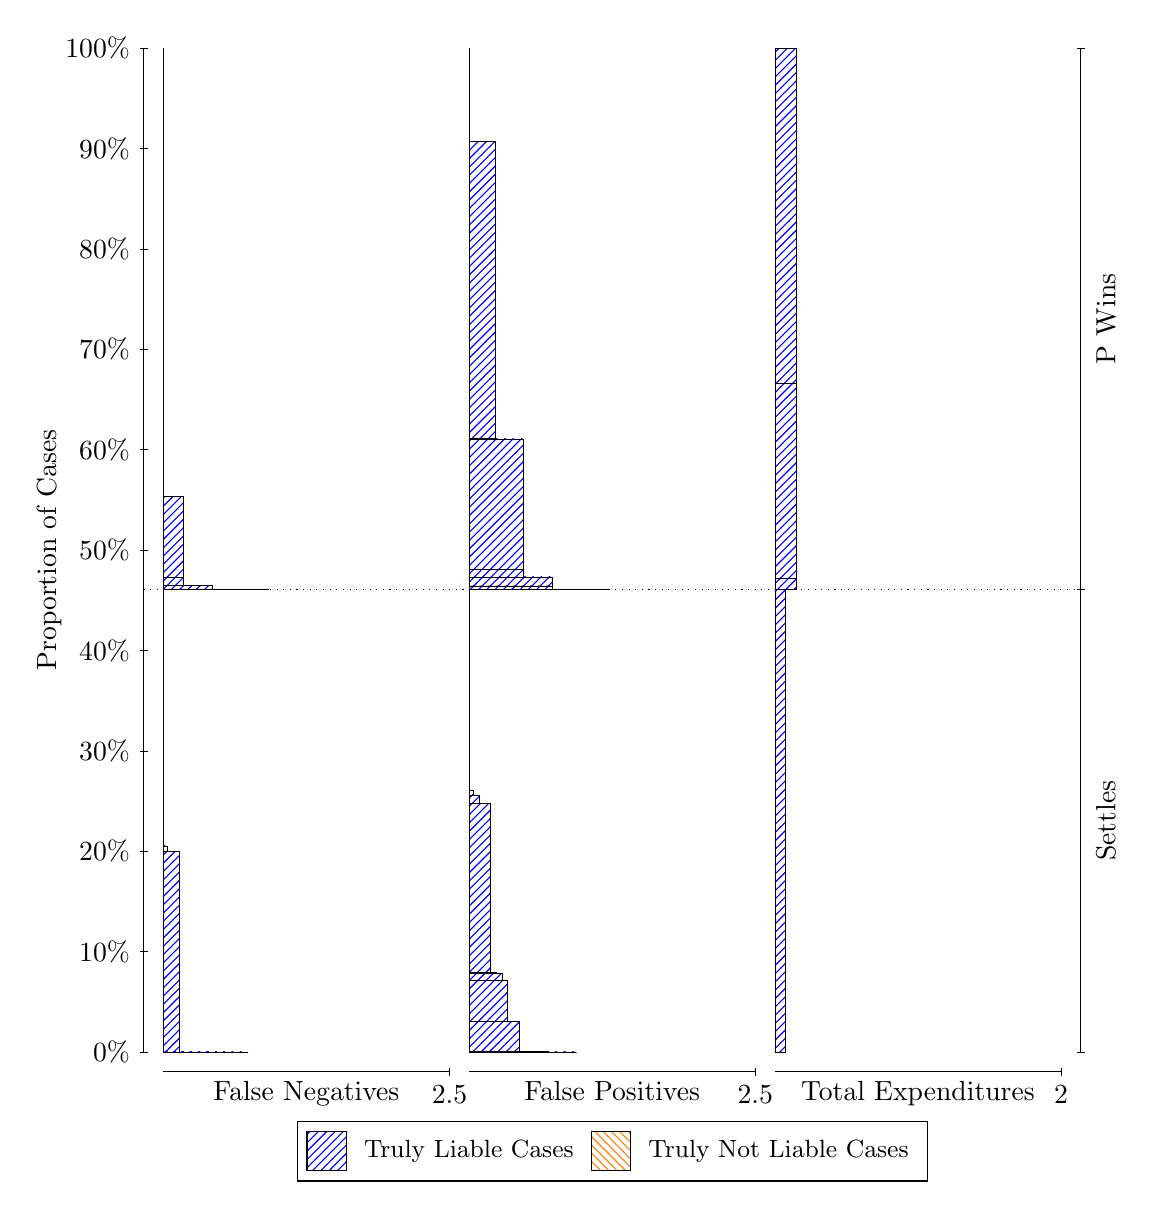
\begin{tikzpicture}
\draw[black, very thin] (1.5,1.75) -- (1.5,14.5);
\node[rotate=90, text=black, anchor=center] at (0.3, 8.125) {Proportion of Cases};
\draw[black, very thin] (1.45,1.75) -- (1.55,1.75);
\node[text=black, anchor=east] at (1.45, 1.75) {0\%};
\draw[black, very thin] (1.45,3.025) -- (1.55,3.025);
\node[text=black, anchor=east] at (1.45, 3.025) {10\%};
\draw[black, very thin] (1.45,4.3) -- (1.55,4.3);
\node[text=black, anchor=east] at (1.45, 4.3) {20\%};
\draw[black, very thin] (1.45,5.575) -- (1.55,5.575);
\node[text=black, anchor=east] at (1.45, 5.575) {30\%};
\draw[black, very thin] (1.45,6.85) -- (1.55,6.85);
\node[text=black, anchor=east] at (1.45, 6.85) {40\%};
\draw[black, very thin] (1.45,8.125) -- (1.55,8.125);
\node[text=black, anchor=east] at (1.45, 8.125) {50\%};
\draw[black, very thin] (1.45,9.4) -- (1.55,9.4);
\node[text=black, anchor=east] at (1.45, 9.4) {60\%};
\draw[black, very thin] (1.45,10.675) -- (1.55,10.675);
\node[text=black, anchor=east] at (1.45, 10.675) {70\%};
\draw[black, very thin] (1.45,11.95) -- (1.55,11.95);
\node[text=black, anchor=east] at (1.45, 11.95) {80\%};
\draw[black, very thin] (1.45,13.225) -- (1.55,13.225);
\node[text=black, anchor=east] at (1.45, 13.225) {90\%};
\draw[black, very thin] (1.45,14.5) -- (1.55,14.5);
\node[text=black, anchor=east] at (1.45, 14.5) {100\%};

\draw[black, very thin] (13.4,1.75) -- (13.4,14.5);
\draw[black, very thin] (13.35,1.75) -- (13.45,1.75);
\node[anchor=west] at (13.35, 1.75) {};
\draw[black, very thin] (13.35,7.6217) -- (13.45,7.6217);
\node[anchor=west] at (13.35, 7.6217) {};
\draw[black, very thin] (13.35,14.5) -- (13.45,14.5);
\node[anchor=west] at (13.35, 14.5) {};

\draw[black, very thin, pattern color=blue, pattern=north east lines] (1.75,1.75) rectangle (2.8218,1.75);
\draw[black, very thin, pattern color=blue, pattern=north east lines] (1.75,1.75) rectangle (2.5312,1.75);
\draw[black, very thin, pattern color=blue, pattern=north east lines] (1.75,1.75) rectangle (2.4585,1.75);
\draw[black, very thin, pattern color=blue, pattern=north east lines] (1.75,1.75) rectangle (2.3858,1.75);
\draw[black, very thin, pattern color=blue, pattern=north east lines] (1.75,1.75) rectangle (2.2405,1.75);
\draw[black, very thin, pattern color=blue, pattern=north east lines] (1.75,1.75) rectangle (2.1678,1.7501);
\draw[black, very thin, pattern color=blue, pattern=north east lines] (1.75,1.7501) rectangle (2.0952,1.7509);
\draw[black, very thin, pattern color=blue, pattern=north east lines] (1.75,1.7509) rectangle (2.0225,1.7509);
\draw[black, very thin, pattern color=blue, pattern=north east lines] (1.75,1.7509) rectangle (1.9498,4.2967);
\draw[black, very thin, pattern color=blue, pattern=north east lines] (1.75,4.2967) rectangle (1.8772,4.2974);
\draw[black, very thin, pattern color=blue, pattern=north east lines] (1.75,4.2974) rectangle (1.8045,4.3665);
\draw[black, very thin, pattern color=orange, pattern=north west lines] (1.75,4.3665) rectangle (1.75,4.3665);
\draw[black, very thin, pattern color=blue, pattern=north east lines] (1.75,4.3665) rectangle (1.75,7.6217);
\draw[black, very thin, pattern color=blue, pattern=north east lines] (1.75,7.6217) rectangle (3.0943,7.6217);
\draw[black, very thin, pattern color=blue, pattern=north east lines] (1.75,7.6217) rectangle (2.731,7.6219);
\draw[black, very thin, pattern color=blue, pattern=north east lines] (1.75,7.6219) rectangle (2.3677,7.622);
\draw[black, very thin, pattern color=blue, pattern=north east lines] (1.75,7.622) rectangle (2.3677,7.6777);
\draw[black, very thin, pattern color=blue, pattern=north east lines] (1.75,7.6777) rectangle (2.0043,7.7741);
\draw[black, very thin, pattern color=blue, pattern=north east lines] (1.75,7.7741) rectangle (2.0043,8.8066);
\draw[black, very thin, pattern color=orange, pattern=north west lines] (1.75,8.8066) rectangle (1.75,8.8066);
\draw[black, very thin, pattern color=blue, pattern=north east lines] (1.75,8.8066) rectangle (1.75,14.5);
\draw[black, very thin, pattern color=orange, pattern=north west lines] (5.6333,1.75) rectangle (6.9958,1.75);
\draw[black, very thin, pattern color=blue, pattern=north east lines] (5.6333,1.75) rectangle (6.9958,1.75);
\draw[black, very thin, pattern color=orange, pattern=north west lines] (5.6333,1.75) rectangle (6.7052,1.75);
\draw[black, very thin, pattern color=blue, pattern=north east lines] (5.6333,1.75) rectangle (6.7052,1.75);
\draw[black, very thin, pattern color=blue, pattern=north east lines] (5.6333,1.75) rectangle (6.6325,1.7526);
\draw[black, very thin, pattern color=orange, pattern=north west lines] (5.6333,1.7526) rectangle (6.5598,1.7526);
\draw[black, very thin, pattern color=blue, pattern=north east lines] (5.6333,1.7526) rectangle (6.5598,1.7526);
\draw[black, very thin, pattern color=orange, pattern=north west lines] (5.6333,1.7526) rectangle (6.4145,1.7526);
\draw[black, very thin, pattern color=blue, pattern=north east lines] (5.6333,1.7526) rectangle (6.4145,1.7536);
\draw[black, very thin, pattern color=blue, pattern=north east lines] (5.6333,1.7536) rectangle (6.3418,1.7543);
\draw[black, very thin, pattern color=blue, pattern=north east lines] (5.6333,1.7543) rectangle (6.2692,2.1427);
\draw[black, very thin, pattern color=blue, pattern=north east lines] (5.6333,2.1427) rectangle (6.1965,2.1429);
\draw[black, very thin, pattern color=orange, pattern=north west lines] (5.6333,2.1429) rectangle (6.1238,2.1429);
\draw[black, very thin, pattern color=blue, pattern=north east lines] (5.6333,2.1429) rectangle (6.1238,2.6602);
\draw[black, very thin, pattern color=blue, pattern=north east lines] (5.6333,2.6602) rectangle (6.0512,2.7446);
\draw[black, very thin, pattern color=blue, pattern=north east lines] (5.6333,2.7446) rectangle (5.9785,2.7607);
\draw[black, very thin, pattern color=blue, pattern=north east lines] (5.6333,2.7607) rectangle (5.9058,4.9049);
\draw[black, very thin, pattern color=blue, pattern=north east lines] (5.6333,4.9049) rectangle (5.8332,4.905);
\draw[black, very thin, pattern color=blue, pattern=north east lines] (5.6333,4.905) rectangle (5.7605,5.0053);
\draw[black, very thin, pattern color=blue, pattern=north east lines] (5.6333,5.0053) rectangle (5.6878,5.0743);
\draw[black, very thin, pattern color=blue, pattern=north east lines] (5.6333,5.0743) rectangle (5.6333,7.6217);
\draw[black, very thin, pattern color=orange, pattern=north west lines] (5.6333,7.6217) rectangle (7.4137,7.6217);
\draw[black, very thin, pattern color=blue, pattern=north east lines] (5.6333,7.6217) rectangle (7.4137,7.6217);
\draw[black, very thin, pattern color=blue, pattern=north east lines] (5.6333,7.6217) rectangle (7.0503,7.6228);
\draw[black, very thin, pattern color=orange, pattern=north west lines] (5.6333,7.6228) rectangle (7.0503,7.6228);
\draw[black, very thin, pattern color=blue, pattern=north east lines] (5.6333,7.6228) rectangle (7.0503,7.6239);
\draw[black, very thin, pattern color=blue, pattern=north east lines] (5.6333,7.6239) rectangle (6.687,7.6703);
\draw[black, very thin, pattern color=orange, pattern=north west lines] (5.6333,7.6703) rectangle (6.687,7.6703);
\draw[black, very thin, pattern color=blue, pattern=north east lines] (5.6333,7.6703) rectangle (6.687,7.7849);
\draw[black, very thin, pattern color=blue, pattern=north east lines] (5.6333,7.7849) rectangle (6.3237,7.8801);
\draw[black, very thin, pattern color=orange, pattern=north west lines] (5.6333,7.8801) rectangle (6.3237,7.8801);
\draw[black, very thin, pattern color=blue, pattern=north east lines] (5.6333,7.8801) rectangle (6.3237,9.5371);
\draw[black, very thin, pattern color=blue, pattern=north east lines] (5.6333,9.5371) rectangle (5.9603,9.5398);
\draw[black, very thin, pattern color=orange, pattern=north west lines] (5.6333,9.5398) rectangle (5.9603,9.5398);
\draw[black, very thin, pattern color=blue, pattern=north east lines] (5.6333,9.5398) rectangle (5.9603,13.315);
\draw[black, very thin, pattern color=blue, pattern=north east lines] (5.6333,13.315) rectangle (5.6333,14.5);
\draw[black, very thin, pattern color=orange, pattern=north west lines] (9.5167,1.75) rectangle (9.6529,1.75);
\draw[black, very thin, pattern color=blue, pattern=north east lines] (9.5167,1.75) rectangle (9.6529,7.6217);
\draw[black, very thin, pattern color=orange, pattern=north west lines] (9.5167,7.6217) rectangle (9.7892,7.6217);
\draw[black, very thin, pattern color=blue, pattern=north east lines] (9.5167,7.6217) rectangle (9.7892,7.7671);
\draw[black, very thin, pattern color=orange, pattern=north west lines] (9.5167,7.7671) rectangle (9.7892,7.7671);
\draw[black, very thin, pattern color=blue, pattern=north east lines] (9.5167,7.7671) rectangle (9.7892,10.245);
\draw[black, very thin, pattern color=orange, pattern=north west lines] (9.5167,10.245) rectangle (9.7892,10.245);
\draw[black, very thin, pattern color=blue, pattern=north east lines] (9.5167,10.245) rectangle (9.7892,14.5);
\draw[black, dotted] (1.5,7.6217) -- (13.4,7.6217);
\draw[black, very thin] (1.75,1.5) -- (5.3833,1.5);
\node[text=black, anchor=north] at (3.5667, 1.5) {False Negatives};
\draw[black, very thin] (5.3833,1.45) -- (5.3833,1.55);
\node[text=black, anchor=north] at (5.3833, 1.45) {2.5};

\draw[black, very thin] (5.6333,1.5) -- (9.2667,1.5);
\node[text=black, anchor=north] at (7.45, 1.5) {False Positives};
\draw[black, very thin] (9.2667,1.45) -- (9.2667,1.55);
\node[text=black, anchor=north] at (9.2667, 1.45) {2.5};

\draw[black, very thin] (9.5167,1.5) -- (13.15,1.5);
\node[text=black, anchor=north] at (11.333, 1.5) {Total Expenditures};
\draw[black, very thin] (13.15,1.45) -- (13.15,1.55);
\node[text=black, anchor=north] at (13.15, 1.45) {2};

\node[text=black, centered, rotate=90] at (13.72, 4.6859) {Settles};
\node[text=black, centered, rotate=90] at (13.72, 11.061) {P Wins};

\draw (7.449999999999999,1.5) node[draw=none] (baseCoordinate) {};
\begin{scope}[align=center]
        \matrix[scale=0.5, draw=black, below=0.5cm of baseCoordinate, nodes={draw}, column sep=0.1cm]{
            \node[rectangle, draw, minimum width=0.5cm, minimum height=0.5cm, pattern color=blue, pattern=north east lines] {}; &
            \node[draw=none, font=\small, text=black] (B) {Truly Liable Cases}; &
            \node[rectangle, draw, minimum width=0.5cm, minimum height=0.5cm, pattern color=orange, pattern=north west lines] {}; &
            \node[draw=none, font=\small, text=black] (B) {Truly Not Liable Cases}; \\
            };
\end{scope}

\end{tikzpicture}
\end{document}